\documentclass[11pt,a4paper]{article}
\usepackage[margin=23mm]{geometry}
\usepackage{amsmath,booktabs,graphicx,siunitx,hyperref}
\title{A ten-bucket example through the optimized CSA}
\date{\today}
\begin{document}\maketitle
The user-provided sequence is 200, 200, 100, 400, 10, 10, 0, 5000, 200, 0 ions.
Buckets last 40 ms. Arrivals are uniform within each bucket, with the paper's
finite-gap current for a 0.5 mm square pad in a grounded plane, 5 mm gap and
constant speed 3 m/s. Its integrated charge is $e[1-\phi_w(g)]$ per ion.
The optimized transistor circuit starts at its quiescent baseline 0.884 V;
its low-charge fitted discharge time is 8.57 s. Five-ms centred averages at
frame boundaries give
\[
 D_n=-[\Delta\overline V_n-\alpha\Delta\overline V_{n-1}],\qquad
 \alpha=\exp(-\Delta t/\tau),\qquad \widehat N_n=D_n/g.
\]
The isolated uniform-packet calibration gives $g=37.98$ $\mu$V per ion.
All following signals are mean noiseless responses. The saved quiescent
noise reference is 75.8 elementary charges RMS per corrected frame.

\begin{table}[ht]\centering
\begin{tabular}{rrrrr}\toprule
Bucket & Collected ions & End voltage (V) & Linear estimate ($e$) & SPICE estimate ($e$)\\\midrule
1 & 200 & 0.876 & 203.5 & 203.5 \\
2 & 200 & 0.868 & 204.7 & 204.7 \\
3 & 100 & 0.864 & 109.9 & 109.9 \\
4 & 400 & 0.849 & 401.7 & 401.2 \\
5 & 10 & 0.849 & 16.2 & 16.2 \\
6 & 10 & 0.848 & 10.2 & 10.1 \\
7 & 0 & 0.848 & 86.9 & 86.8 \\
8 & 5000 & 0.654 & 5003.5 & 4970.6 \\
9 & 200 & 0.647 & 275.1 & 271.2 \\
10 & 0 & 0.648 & 3.0 & 2.5 \\
\bottomrule\end{tabular}
\caption{Raw voltage at each boundary and charge inferred from the centred
averages with the fixed low-charge gain. Both estimates retain the response
spreading between adjacent buckets.}\end{table}

For this sequence the circuit remains close to the linear prediction.
The 5000-ion deposit does not drive it into the strongly compressed regime seen
in the extreme event histories. Earlier charge remains on the CSA as each
bucket arrives; the output therefore decreases across the occupied buckets and
recovers gradually after collection.

Bucket 7 has zero collected ions but a positive estimated signal from ions
collected in bucket 8. Induction begins before collection, and the centred
averaging window also extends across the boundary. Bucket 9 includes signal
from the large deposit as well as its own 200 ions. These deterministic adjacent
responses must be included when converting frame estimates to collected counts.

Paired controls remove the bucket-9 deposit while keeping the rest of the
history fixed. The marginal estimated contribution of its 200 ions is 197.4
with the large deposit present. Removing the 5000-ion deposit and repeating the
same paired comparison gives 199.7. The relative reduction of the
marginal response is 1.13\%.

\begin{figure}[ht]\centering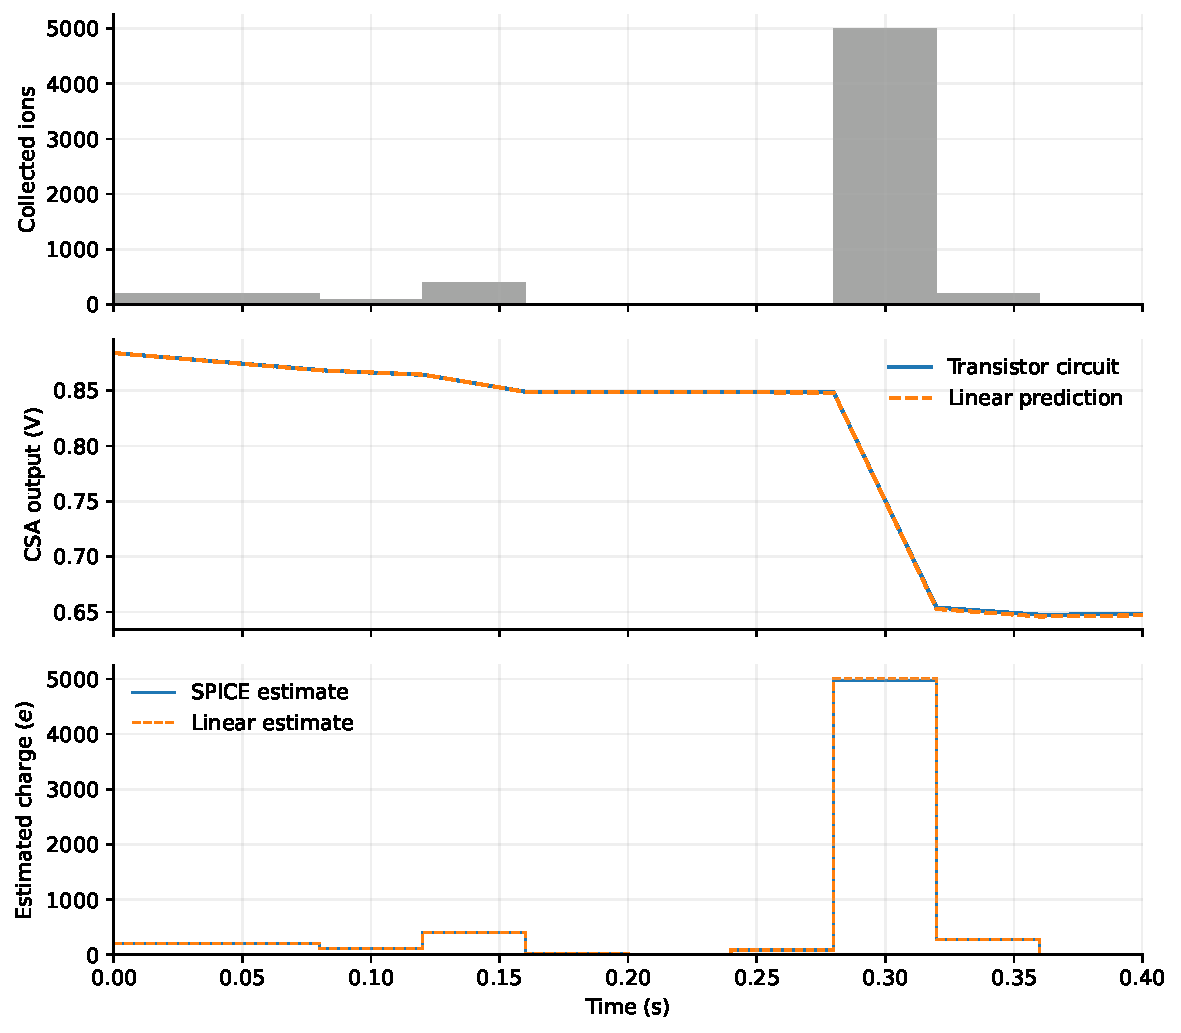
\includegraphics[width=.95\linewidth]{sequence.pdf}
\caption{The complete sequence retains the accumulated CSA state. The linear
and transistor-level predictions nearly coincide at this charge scale.}
\end{figure}

\paragraph{Validation and reproduction.}
Four histories (requested sequence, removal of bucket 9, removal of bucket 8,
and removal of both) are simulated at two resolutions with matched zero-input
references. Eight PWL charge checks and eight transient charge/refinement
checks pass. Configuration, code, model, simulator and netlist hashes are saved
with HDF5 outputs in \texttt{results/ltspice/pad\_sequence\_example/}.
Julia performs current generation and reduction; Python acquires SPICE output
and presents the HDF5 results. From the repository root:
\begin{verbatim}
PYTHONPATH=src python scripts/run_pad_sequence_example.py \
  --simulator /path/to/LTspice
python scripts/present_pad_sequence_example.py
\end{verbatim}
The report source is generated without compiling the PDF.
\end{document}
